\section{Related Work}

\paragraph{Long-Term Dialogue Benchmarks} {As the ability of dialogue systems improve, research starts to focus on long-term dialogue understanding beyond traditional dialogue modeling benchmarks \citep{budzianowski-etal-2018-multiwoz, wei-etal-2018-airdialogue}.} Early works focused on language modeling evaluation on generating personalized responses from human-human \citep{xu-etal-2022-beyond} or human-AI \citep{xu-etal-2022-long} chat histories. To more precisely evaluate memory accuracy, subsequent benchmarks shifted toward question answering (QA, \citet{reddy-etal-2019-coqa, zhang-choi-2021-situatedqa}). For example, MemoryBank \citep{zhong2024memorybank} features multi-day chat histories from 15 users with 194 human-written probing questions. LoCoMo \citep{maharana-etal-2024-evaluating} includes 50 long-term chat histories and questions testing single-hop, multi-hop, temporal, commonsense, world knowledge, and adversarial reasoning. PerLTQA \citep{du-etal-2024-perltqa} scales the evaluation to 3,409 dialogues and 8,593 questions, covering world knowledge, personal profiles, social relationships, events, and dialogue history. DialSim \citep{kim2024dialsimrealtimesimulatorevaluating} evaluates models' memory ability by roleplaying TV show characters and introduces a time constraint that penalizes slow system responses. Despite these advancements, existing QA-based benchmarks overlook several memory capabilities critical to long-term user-assistant interactions: synthesizing information across numerous sessions, recalling assistant side information, and reasoning about updated user details or complex temporal references. Additionally, the chat histories are often too brief and do not reflect the nature of task-oriented interactions. \Cref{tab:benchmark-comparison} compares between \BENCHMARK{} and previous works, highlighting its advantages in both (1) featuring a long and freely extensible iterative history and (2) holistically covering critical memory abilities in a uniquely challenging way (further examples in \Cref{fig:main-fig-benchmark-examples}). 

\setlength{\tabcolsep}{3.3pt}
\begin{table}[t!]{
\centering
\vspace{-2mm}
\caption{A comparison between \BENCHMARK{} and existing long-term memory benchmarks. We use different colors to denote \textcolor{teal}{human-human} and \textcolor{violet}{human-AI} dialogue. \#Sess and \#Q denote the total number of sessions and questions. Context depth is defined as the number of tokens in the history. Finally, we compare the coverage of five core abilities: information extraction (IE), multi-session reasoning (MR), knowledge update (KU), temporal reasoning (TR), and abstaining on unanswerable questions (ABS). $^{*}$Not reported in the paper, based on our approximation.  $^{**}$at most 2 sessions.}
\vspace{-2mm}
\resizebox{0.92\linewidth}{!}{
\centering
\begin{tabular}{l|c|c|c|c|c|c|c|c|c}
\hline
\multirow{2}{*}{\textbf{Benchmark}} & \multirow{2}{*}{\textbf{Domain}} & \multirow{2}{*}{\textbf{\#Sess}} & \multirow{2}{*}{\textbf{\#Q}} & \multirow{2}{*}{\textbf{Context Depth}} & \multicolumn{5}{c}{\textbf{Core Memory Abilities}} \\ 
% \cline{6-10}
 &  &  &  &  & \multicolumn{1}{c}{\textbf{IE}} & \multicolumn{1}{c}{\textbf{MR}} & \multicolumn{1}{c}{\textbf{KU}} & \multicolumn{1}{c}{\textbf{TR}} & \multicolumn{1}{c}{\textbf{ABS}} \\ 
\hline
MSC \citep{xu-etal-2022-beyond} & \textcolor{teal}{Open-Domain} &  5k & - &  1k & \ding{55} & \ding{55} & \ding{55} & \ding{55} & \ding{55} \\
DuLeMon \citep{xu-etal-2022-long} & \textcolor{violet}{Open-Domain} &  30k & - &  1k & \ding{55} & \ding{55} & \ding{55} & \ding{55} & \ding{55} \\
MemoryBank \citep{zhong2024memorybank} & \textcolor{violet}{Personal} & 300 & 194 &  5k & \checkmark & \ding{55} & \ding{55} & \checkmark & \ding{55} \\
PerLTQA \citep{du-etal-2024-perltqa}& \textcolor{violet}{Personal} &  4k & 8593 &  1M$^*$ & \checkmark & \ding{55} & \ding{55} & \ding{55} & \checkmark \\
LoCoMo \citep{maharana-etal-2024-evaluating} & \textcolor{teal}{Personal} &  1k & 7512 &  10k & \checkmark & \checkmark & \ding{55} & \checkmark & \checkmark \\
DialSim \citep{kim2024dialsimrealtimesimulatorevaluating} & \textcolor{teal}{TV Shows} & 1k–2k &  1M &  350k & \checkmark & \checkmark$^{**}$ & \ding{55} & \checkmark & \checkmark \\
\BENCHMARK{} (this work) & \textcolor{violet}{Personal} &  50k & 500 &  115k,  1.5M & \checkmark & \checkmark & \checkmark & \checkmark & \checkmark \\
\hline
\end{tabular}
}
\label{tab:benchmark-comparison}
}
\end{table}

\begin{figure}[t!]
 \centering
 \vspace{-1mm}
 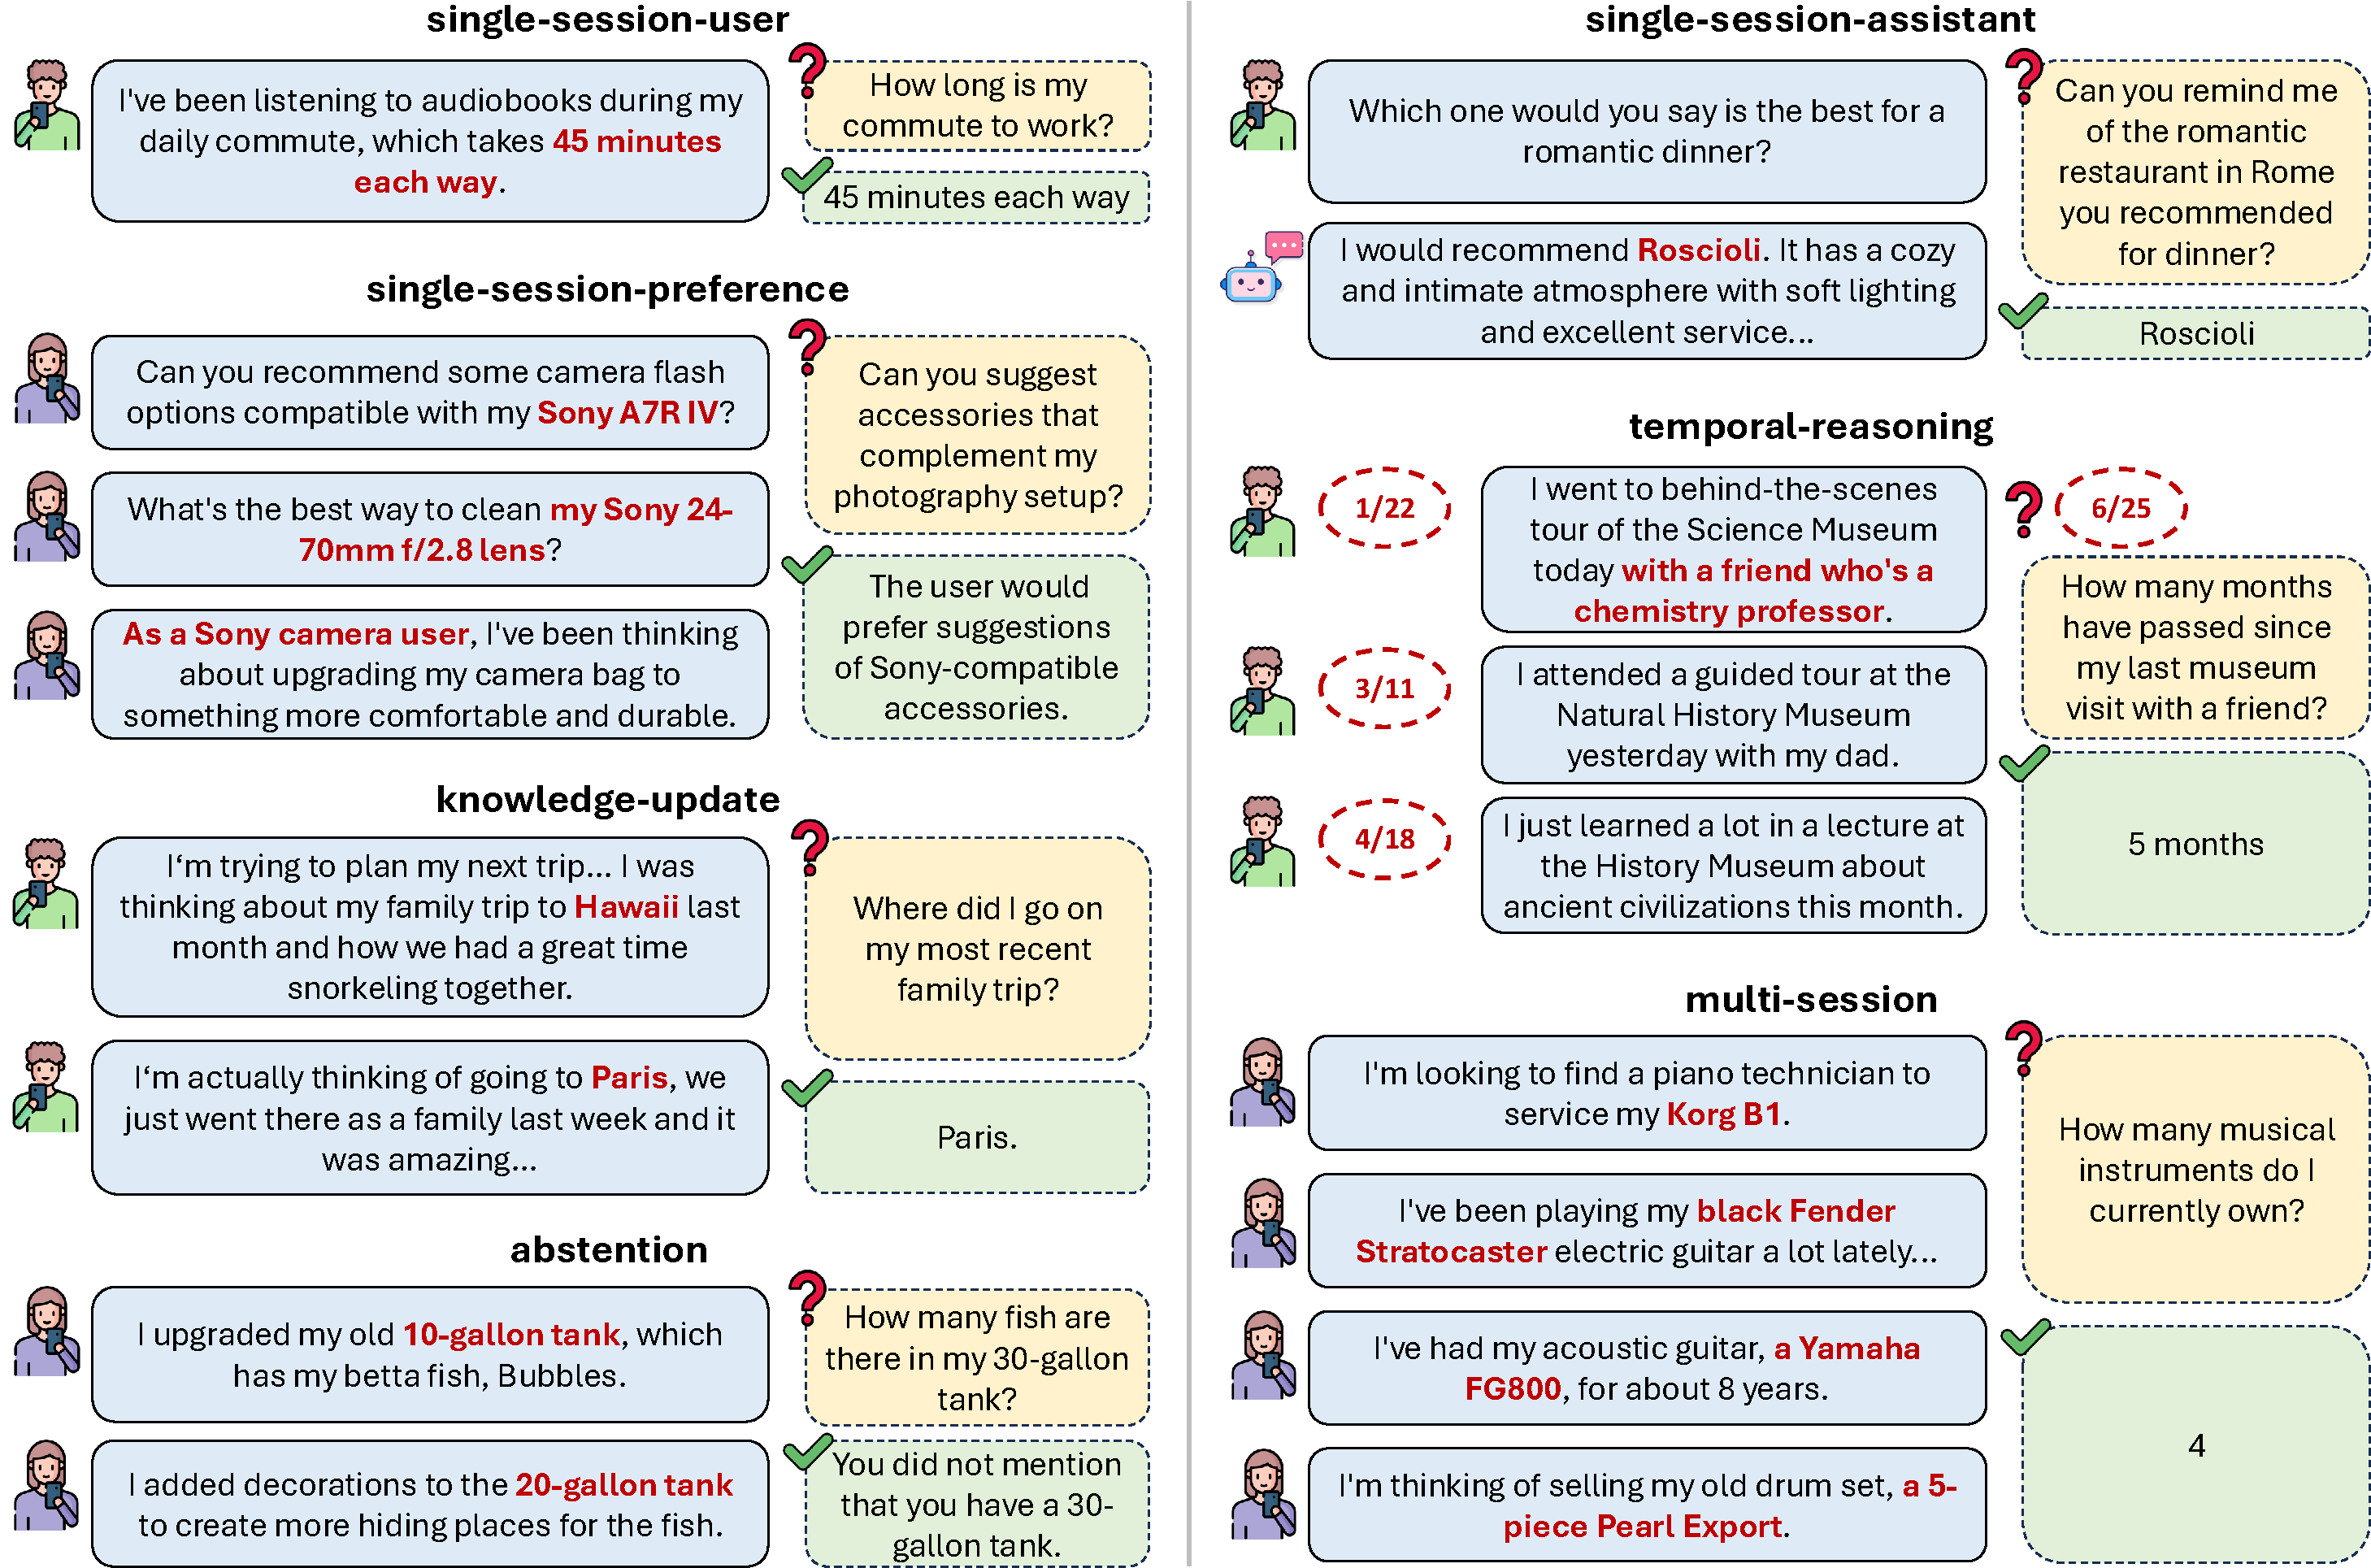
\includegraphics[width=0.95\textwidth]{figures/main_examples.pdf}
 \vspace{-1mm}
 \caption{Examples of the seven question types in \BENCHMARK{}. For each example, we show the associated evidence statements on the left and the question with the answer on the right.}
 \label{fig:main-fig-benchmark-examples}
\vspace{-5mm}
\end{figure}

\paragraph{Long-Term Memory Methods} To equip chat assistants with long-term memory capabilities, three major techniques are commonly explored. The first approach involves directly adapting LLMs to process extensive history information as long-context inputs \citep{Beltagy2020Longformer,kitaev2020reformer,DBLP:conf/icml/FuPNYHK024,DBLP:journals/corr/abs-2404-16811}. While this method avoids the need for complex architectures, it is inefficient and susceptible to the ``lost-in-the-middle" phenomenon, where the ability of LLMs to utilize contextual information weakens as the input length grows \citep{DBLP:conf/icml/ShiCMSDCSZ23, DBLP:journals/tacl/LiuLHPBPL24}. A second line of research integrates differentiable memory modules into language models, proposing specialized architectural designs and training strategies to enhance memory capabilities \citep{weston2014memory, wu2022memorizing, zhong-etal-2022-training, DBLP:conf/nips/Wang0CLYGW23}. Lastly, several studies approach long-term memory from the perspective of context compression, developing techniques to condense lengthy histories into compact representations, whether in the form of LLM internal representations \citep{DBLP:conf/nips/Mu0G23, DBLP:conf/emnlp/ChevalierWAC23}, discrete tokens \citep{DBLP:conf/emnlp/JiangWLYQ23, DBLP:conf/iclr/XuSC24}, or retrievable text segments via retrieval-augmented generation (RAG, \citet{shi-etal-2024-replug, DBLP:conf/nips/Wang0CLYGW23, DBLP:conf/iclr/SarthiATKGM24, DBLP:journals/corr/abs-2310-05029, DBLP:journals/corr/abs-2405-14831}). Although \BENCHMARK{} can evaluate any memory system, we will take an online context compression perspective, where each history interaction session is sequentially processed, stored, and accessed on-demand through indexing and retrieval mechanisms (\Cref{section-unified-view}). This formulation aligns with current literature \citep{zhong2024memorybank,DBLP:journals/corr/abs-2405-14831} and commercial systems \citep{openai_memory_2024, coze_memory_2024}. Its plug-and-play nature also facilitates the integration into existing chat assistant systems. 

